
\subsubsection{menuconfig}\label{menuconfig}
    Dieses Paket verwaltet die Konfigurationsdateien für alle 
    Einstellungen, die im Einstellungsfenster des Menüs vorgenommen werden können.
    Dabei existiert für jede Dateei eine eigene Klasse. In den Klassen wird
    keine Einstellung durch den Benutzer vorgenommen. Es existieren lediglich
    Methoden, um die aktuellen eventuell veränderten Änderungen in die Datei 
    zu schreiben. Ebenfalls können die aktuell gespeicherten Dateien geladen
    und den anderen Klassen zur Verfügung gestellt werden. \par

    \begin{figure}[!h]
        \centering
        \centering
            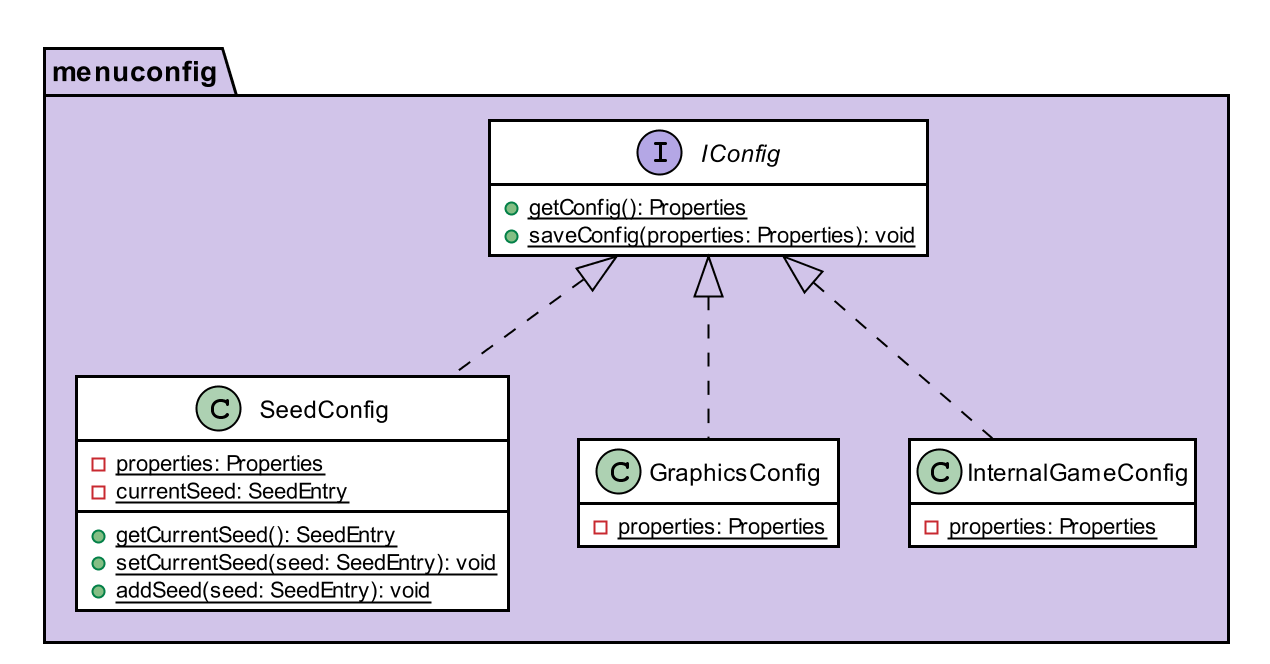
\includegraphics[width=\linewidth]{./GUI/GUI_Bilder/Config.png}
              \caption{Paket menuconfig}
               \label{fig:Config}
    \end{figure}

        \paragraph{\underline{IConfig}}\label{configlabel} \mbox{}\\
            Dieses Interface stellt Funktionen bereit, um Dateien zu laden und zu speichern.
            Jede Klasse die dieses Interface implementiert, muss die beiden Funktionen 
            überschreiben.

            \textbf{Methoden}					
            \begin{itemize}
                \item \textit{+ {static} getConfig(): Properties}
                    \begin{leftbar}[0.9\linewidth]
                        Gibt das Properties Objekt der Konfiguration zurück.\\
                        \textbf{@return} Das aktuelle Properties Objekt.
                    \end{leftbar}
                \item \textit{+ {static} saveConfig(Properties properties): void}
                    \begin{leftbar}[0.9\linewidth]
                        Überschreibt das aktuelle Properties Objekt mit dem übergebenem.\\
                        \textbf{@param properties} Das zu speichernde Properties Objekt.
                    \end{leftbar}
            \end{itemize}
            \pagebreak
        \paragraph{\underline{SeedConfig}} \mbox{}\\
            Diese Klasse verwaltet die Konfiguration der Seeds, bzw. speichert alle 
            vorhandenen Seeds in einer Datei, oder ergänzt diese um einen Seed. 
            Außerdem speichert sie den aktuell ausgewählten Seed.
            Ebenfalls wird das Interface~\nameref{configlabel} implementiert, um die Konfigurations Datei
            laden und speichern zu können. \par 
            \textbf{Attribute}
            \begin{itemize}
                \item \textit{- {static} Properties properties}
                    \begin{leftbar}[0.9\linewidth]
                        In diesem Properties Objekt werden die Einstellungen bzw Daten 
                        gespeichert.
                    \end{leftbar}
                \item \textit{- {static} currentSeedEntry: SeedEntry} 
                    \begin{leftbar}[0.9\linewidth]
                        Enthält den aktuell ausgewählten Seed.
                    \end{leftbar}
            \end{itemize}
            
            \textbf{Methoden}					
            \begin{itemize}
                \item \textit{+ {static} getCurrentSeed(): SeedEntry}
                    \begin{leftbar}[0.9\linewidth]
                        Gibt den aktuell ausgewählten Seed zurück.\\
                        \textbf{@return} Der aktuell ausgewählte Seed.
                    \end{leftbar}
                \item \textit{+ {static} setCurrentSeed(SeedEntry seed): void}
                    \begin{leftbar}[0.9\linewidth]
                        Überschreibt den aktuellen Seed mit einem neuen Seed Objekt.\\
                        \textbf{@param seed} Der zu speichernde Seed.
                    \end{leftbar}
                \item \textit{+ {static} addSeed(SeedEntry seed): void}
                    \begin{leftbar}[0.9\linewidth]
                        Fügt der SeedConfig Datei einen neuen Seed hinzu, wobei die 
                        Alten beibehalten werden.\\
                        \textbf{@param seed} Der Seed welcher hinzugefügt werden soll.
                    \end{leftbar}
            \end{itemize}

        \pagebreak
        \paragraph{\underline{GraphicsConfig}} \mbox{}\\
            Diese Klasse verwaltet die Konfiguration der im Menü einstellbaren 
            Grafikeinstellungen, bzw. speichert alle vorgenommen Änderungen der
            Grafik in einer Datei. 
            Ebenfalls wird das Interface~\nameref{configlabel} implementiert, um die Konfigurations Datei
            laden und speichern zu können. \par    
                    
            \textbf{Attribute}
            \begin{itemize}
                \item \textit{- {static} Properties properties}
                    \begin{leftbar}[0.9\linewidth]
                        In diesem Properties Objekt werden die Einstellungen bzw Daten 
                        gespeichert.
                    \end{leftbar}
            \end{itemize}
            
            \textbf{Methoden}					
            \begin{itemize}
                \item \textit{+ {static} getGraphicsConfig(): Properties}
                    \begin{leftbar}[0.9\linewidth]
                        Gibt das Properties Objekt der Grafik Konfiguration zurück.\\
                        \textbf{@return} Das aktuelle Properties Objekt.
                    \end{leftbar}
            \end{itemize}
		
		\paragraph{\underline{InternalGameConfig}} \mbox{}\\
            Diese Klasse verwaltet die Konfiguration der im Menü einstellbaren 
            internen Spieleinstellungen, bzw. speichert alle vorgenommen Änderungen
            in einer Datei. 
            Ebenfalls wird das Interface~\nameref{configlabel} implementiert, um die Konfigurations Datei
            laden und speichern zu können. \par    
                    
            \textbf{Attribute}
            \begin{itemize}
                \item \textit{- {static} Properties properties}
                    \begin{leftbar}[0.9\linewidth]
                        In diesem Properties Objekt werden die Einstellungen bzw Daten 
                        gespeichert.
                    \end{leftbar}
            \end{itemize}

    \pagebreak